\documentclass[main.tex]{subfiles}
\begin{document}
\chapter{Existing many-core COTS processors}

\section{\mppalong}
As depicted in figure~\ref{fig_stateOfTheArt_mppa_overview}, the \mppalong~\cite{kalray_mppa} integrates 288 cores distributed over 16 compute clusters and 4 I/O clusters . All the clusters are interconnected by two parallel Networks-on-Chip having a 2D-torus topology. %(only one of the two NoCs is depicted in figure~\ref{fig_stateOfTheArt_mppa_noc_overview} for clarity).
Each compute cluster essentially features:
\begin{itemize}
    \item 16 cores denoted as the \emph{Processing Elements} (or \emph{PEs}) dedicated to run user code. Each PE has private instruction and data caches of 8KiB each with no hardware support to enforce cache coherency inside a cluster. 
    \item 1 additional core denoted as the \emph{Resource Manager} (or \emph{RM}) which only differs from the PEs by its privileged accesses to the configuration registers of the cluster.
    \item 2 NoC interfaces (one for each NoC).
    \item 1 Direct Memory Access unit (or \emph{DMA}) capable of pushing and receiving data through the NoC interface.
    \item 2MiB of of Static Random Access Memory (or \emph{SRAM}) divided into 16 independent banks of equal size that are accessible only by the local elements of the cluster. Any read of write request targeting the SRAM of different cluster must be performed by explicit message passing through the NoC using the DMA unit.
\end{itemize}

Each I/O cluster is composed of 4 RMs with private instruction caches and a single shared data cache, 512 KiB of SRAM in a single bank, 8 NoC interfaces (4 per NoC), 4 DMA controllers and no PE. Moreover, unlike the compute clusters, the I/O clusters have access to additional peripherals such as the DDR-SDRAM or Ethernet controllers. Consequently, all the requests initiated by a PE (and thus necessarily from a compute cluster) and targeting out-of-chip components must be performed by explicit message passing on the NoC between the compute and the I/O cluster.


Although sharing the same topology and the same flow control strategy based on wormhole switching, the two NoCs, denoted as the Data-NoC (or \emph{D-NoC}) and the Control-NoC (or \emph{C-NoC}), have been designed for different purposes. The D-NoC is dedicated to the transfer or large chunks of data. It provides QoS mechanisms using hardware limiters enabling the regulation of the injected traffic under $(\rho , \sigma)$ constraints~\cite{deDinechin2014NoCArc}. On the other hand, the C-NoC enables inter-cluster synchronizations thanks to short control messages and barrier mechanisms. 

All the 288 cores have the same 5-issue VLIW~\cite{Fisher1983} instruction set architecture (or \emph{ISA}) with a 7-stage instruction pipeline. In the context of the \certainty project~\cite{Certainty}, the cores of the \mppalong have been proven to have the property of \emph{full timing compositionality}~\cite{Certainty:D33} by \absint~\cite{AbsInt}. 

Overall, the major architectural traits of the MPPA such as: 1) the VLIW ISA of the cores; 2) the absence of hardware support for cache coherency; and 3) the need of explicit message passing to achieve inter-cluster communication and out-of-chip transactions enable both a very power efficient implementation of the chip (in terms of flops per watt) and a fine-grained management of shared resources by software. Nonetheless, these two very desirable properties in the context of hard real-time embedded systems come at the price of a largely increased programming complexity.

\begin{figure}
    \centering
    %\scalebox{1.5}{\input{imgs/tex/all_MPPA_NoC_overview.tex}}
    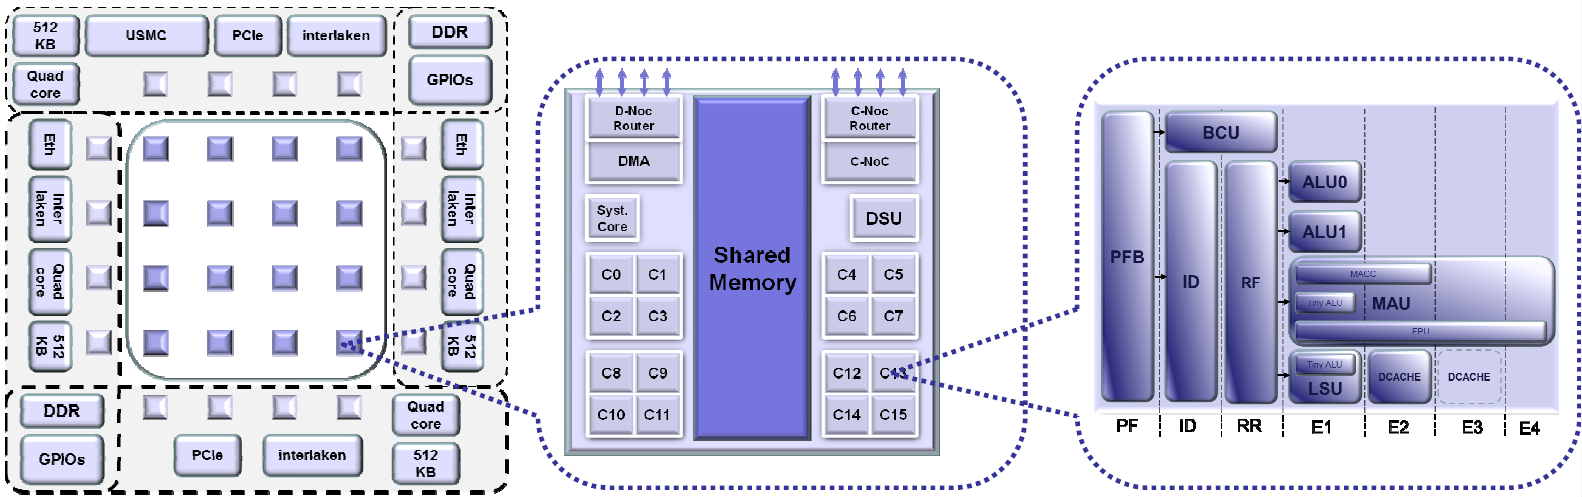
\includegraphics[width=16cm]{imgs/png/all_MPPA_nested_overview.png}
    \caption{Architecture of the \mppalong (extracted from~\cite{kalray_slides_irit})}
    \label{fig_stateOfTheArt_mppa_overview}
\end{figure}


\section{Mellanox TILE-Gx family}
Although distributed by Mellanox Technologies, the TILE-Gx36 and TILE-Gx72 processors were originally designed by Tilera Corporation (acquired in 2014 by EZchip Semiconductor which was later acquired by Mellanox in early 2016) to target mainly the markets of networking equipments and multimedia applications.

As depicted in figure~\ref{fig_stateOfTheArt_TILEGx72_overview}, a TILE-Gx72 processor features 72 cores (36 in a TILE-Gx36) each of which is encapsulated in a \emph{tile}. All the 72 (or 36) tiles are interconnected by 5 parallel NoCs.
All tiles are identical and include:
\begin{itemize}
    \item a 64-bit VLIW processing core clocked at 1.2GHz;
    \item a 32 KiB 2-way set associative L1 cache for data;
    \item a 32 KiB 2-way set associative L1 cache for instruction;
    \item a 256 KiB 8-way set associative unified \emph{coherent}\footnotemark L2 cache that can be configured to handle misses using 3 different page homing policies;
    \item and a switch managing the 5 NoCs.
\end{itemize}
\footnotetext{The set of all the L2 caches are coherent and can thus be seen as a large virtual cache from a developer point of vue. This distributed cache is often referred to as the L3 cache in the TILE-Gx's documentation although there are no physical existence of such a third level of cache.}

The tiles are surrounded by several I/O peripherals such the 4 DDR controllers, or the 8 Ethernet interfaces. All these I/O interfaces are accessible from the tiles through the NoCs.

The 5 NoCs have the same 2D-mesh topology, the same flow control mechanism (wormhole switching) and the same default routing strategy (x-first, which can be changed to y-first by configuration). However they belong to two different classes. The first class includes two software accessible NoCs denoted as the User Dynamic Network (or \emph{UDN}) and the I/O Dynamic Network (or \emph{IDN}). The typical usage of the UDN is to enable application level communications between tiles while the IDN is essentially used for OS or hypervisor operations.

The second class includes three NoCs that are invisible from software: the reQuest Dynamic Network (or \emph{QDN}), the Response Dynamic Network (or \emph{RDN}) and the Share Dynamic Network (or \emph{SDN}). Both the QDN and the RDN handle external memory transactions. The SDN is used to ensure the coherency between the L2 caches.


\begin{figure}
    \centering
    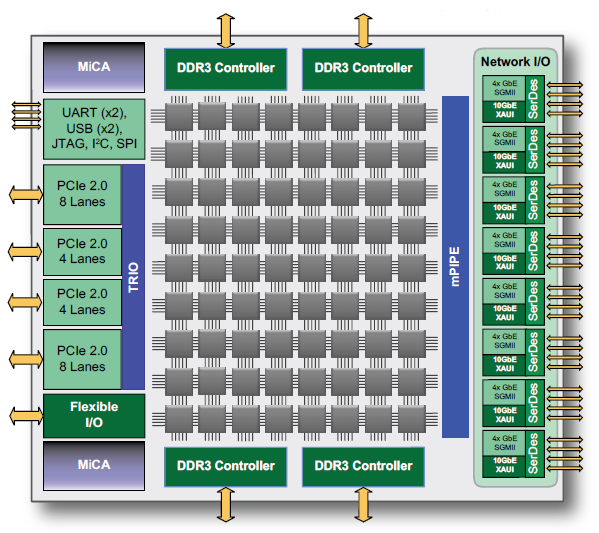
\includegraphics[height=9cm]{imgs/png/stateOfTheArt_TILEGx72_overview.png}
    \caption{Architecture of the TILE-Gx8072 processor (extracted from~\cite{TileGx})}
    \label{fig_stateOfTheArt_TILEGx72_overview}
\end{figure}



\section{Intel Single-chip Cloud Computer (SCC)}
The Intel Single-chip Cloud Computer (or \emph{SCC}) is a many-core processor used for experimental and research purposes only~\cite{intel_scc}. As shown on figure~\ref{fig_stateOfTheArt_IntelSCC_overview}, it comprises 24 dual-core tiles interconnected via a $6 \times 4$ mesh NoC. The cores are based on a Pentium IA-32 instruction set and features 16KiB of instruction cache and respectively 16KiB and 256KiB of L1 and L2 data caches each. However, there are no hardware enforced cache coherency. 

The NoC communications are always routed with the x-first policy at the packet granularity. The inter-tile exchange of data can be done either using the external main memory or directly via a tile-to-tile communication over the NoC if the data size is less than the 16KiB of a Message Passing Buffer (or \emph{MPB}). 
The NoC is also connected to 4 DDR3-SDRAM controllers enabling up to 64 GiB of external memory and to a System Interface (or \emph{SIF}) offering external access to the NoC through a simple parallel bus. The SIF can be leveraged to add complex I/Os such as PCIe, Ethernet or SATA.

The SCC enables rather fine-grained configurations of both frequency and voltage scaling. The voltage adjustments can be done on groups of 4 tiles while the frequency adjustments can be done at the tile level. Overall, these power management mechanisms can lead to drop the energy consumption from 125W to 25W in specific circumstances~\cite{Howard2010}.


\begin{figure}
    \centering
    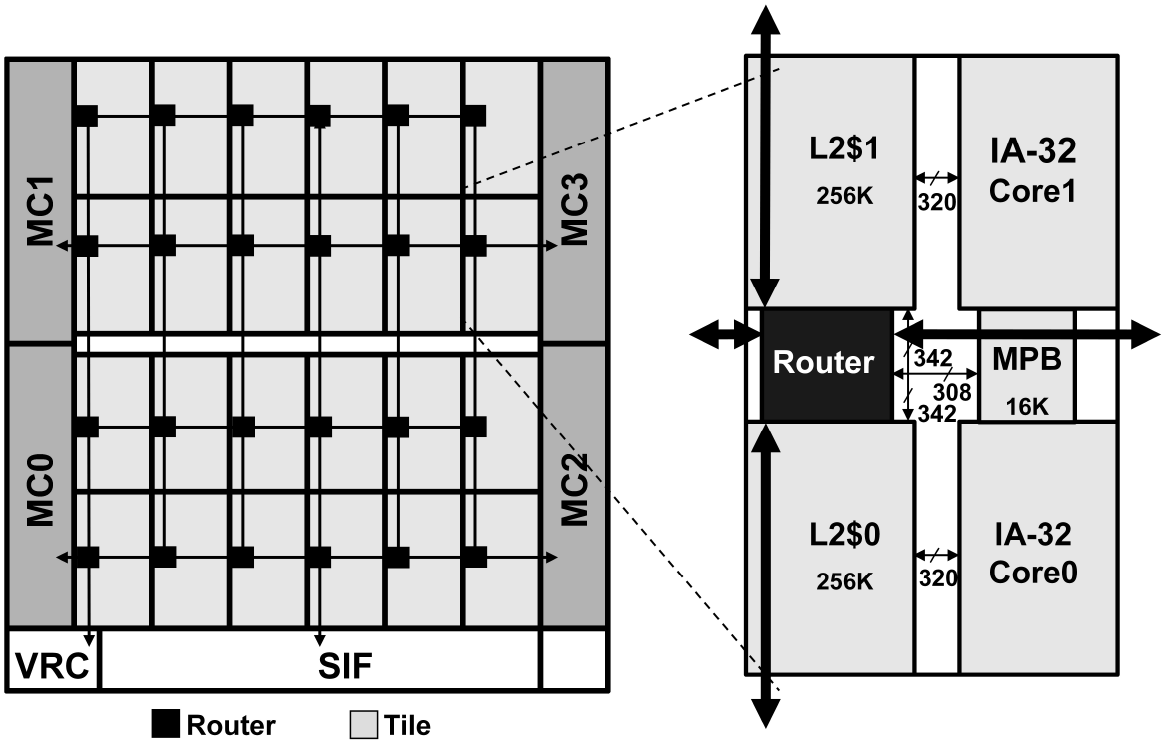
\includegraphics[width=10cm]{imgs/png/stateOfTheArt_IntelSCC_overview.png}
    \caption{Architecture of the Intel SCC processor (extracted from~\cite{Howard2010})}
    \label{fig_stateOfTheArt_IntelSCC_overview}
\end{figure}






\section{Compatibility with an avionics context}
\subsection{Time-predictability}
\subsection{Availability of informations}
\subsection{Power consumption}
Passive cooling of electronics is an important asset to enable the certification of avionics boards. Indeed ... \textbf{a completer une fois avec les valeurs}.
The thermal resistance of the required heat sink $\Theta_{sa}$ can be deduced from the thermal Ohm's law~\cite{Edmunds_heatsinks} as in equation~\ref{eq_stateOfTheArt_therman_resistance}.

\begin{equation}
    \label{eq_stateOfTheArt_therman_resistance}
    \Theta_{sa} = \dfrac{T_j - T_a}{Q} - (\Theta_{jc} + \Theta_{cs})
\end{equation}
with $T_j$ the junction temperature (in \degree C), $T_a$ the ambient fluid temperature (in \degree C), $Q$ the power dissipation (in W), $\Theta_{jc}$ the junction-to-case thermal resistance (in \degree C / W) and $\Theta_{cs}$ the thermal resistance of the thermal grease in between the case and the heatsink. 

We assume $T_a = 70 $ \degree C corresponding to the \emph{Operating High Temperature} for testing equipments as specified in the DO160~\cite{do160}.





\end{document}
